\documentclass[3p]{elsarticle} %review=doublespace preprint=single 5p=2 column
%%% Begin My package additions %%%%%%%%%%%%%%%%%%%

\usepackage[hyphens]{url}


\usepackage{lineno} % add
  \linenumbers % turns line numbering on

\usepackage{graphicx}
%%%%%%%%%%%%%%%% end my additions to header

\usepackage[T1]{fontenc}
\usepackage{lmodern}
\usepackage{amssymb,amsmath}
\usepackage{ifxetex,ifluatex}
\usepackage{fixltx2e} % provides \textsubscript
% use upquote if available, for straight quotes in verbatim environments
\IfFileExists{upquote.sty}{\usepackage{upquote}}{}
\ifnum 0\ifxetex 1\fi\ifluatex 1\fi=0 % if pdftex
  \usepackage[utf8]{inputenc}
\else % if luatex or xelatex
  \usepackage{fontspec}
  \ifxetex
    \usepackage{xltxtra,xunicode}
  \fi
  \defaultfontfeatures{Mapping=tex-text,Scale=MatchLowercase}
  \newcommand{\euro}{€}
\fi
% use microtype if available
\IfFileExists{microtype.sty}{\usepackage{microtype}}{}
\usepackage[]{natbib}
\bibliographystyle{plainnat}

\ifxetex
  \usepackage[setpagesize=false, % page size defined by xetex
              unicode=false, % unicode breaks when used with xetex
              xetex]{hyperref}
\else
  \usepackage[unicode=true]{hyperref}
\fi
\hypersetup{breaklinks=true,
            bookmarks=true,
            pdfauthor={},
            pdftitle={Nest shape influences colony organization in ants: colony spatial distribution differs from random movement},
            colorlinks=false,
            urlcolor=blue,
            linkcolor=magenta,
            pdfborder={0 0 0}}

\setcounter{secnumdepth}{0}
% Pandoc toggle for numbering sections (defaults to be off)
\setcounter{secnumdepth}{0}


% tightlist command for lists without linebreak
\providecommand{\tightlist}{%
  \setlength{\itemsep}{0pt}\setlength{\parskip}{0pt}}




\usepackage{parskip}

\begin{document}


\begin{frontmatter}

  \title{Nest shape influences colony organization in ants: colony
spatial distribution differs from random movement}
    \author[a]{Greg T. Chism}
   \ead{gchism@arizona.edu} 
    \author[b]{William Nichols}
  
    \author[c]{Anna Dornhaus}
  
      \affiliation[a]{Graduate Interdisciplinary Program in Entomology
and Insect Science, University of Arizona, Tucson, AZ, U.S.A.}
    \affiliation[b]{School of Plant Sciences, University of Arizona,
Tucson, AZ, U.S.A.}
    \affiliation[c]{Department of Ecology and Evolutionary Biology,
University of Arizona, Tucson, AZ, U.S.A.}
    \cortext[cor1]{Corresponding author}
  
  \begin{abstract}
  Many social animals produce architectures that greatly increase the
  builder's ability to survive across environments. For example, the
  many forms and functions of ant nests facilitate their ability to
  occupy nearly every biome. However, nest shape is not always
  determined by the ants, as some species inhabit cavities with
  externally determined shapes, such as rock crevices or hollow sticks.
  In both cases, we can ask not only how ant behaviour can affect the
  form and function of nests, but also how nest shapes impact the
  inhabiting ant colony's behaviour. We examined how the spatial
  organization of \emph{Temnothorax rugatulus} ants differed across
  given artificial nests with radically different internal shapes. We
  used geometric measures to describe the emerging spatial relationships
  of workers, brood, queens, and alates in these two shapes, and show
  that overall distributions of all types of colony members are
  influenced by nest shape. However, we also found that individual
  spatial fidelity zone size, i.e.~the areas repeatedly occupied by
  individuals, which may be linked to their division of labor, are
  overall not affected by nest shape. This is even though spatial
  fidelity zone size does vary as a function of distance from the nest
  entrance and brood center; and that this relationship is affected by
  both nest shape and density. Finally, we show that workers are found
  closer to the nest entrance than would be expected in a random walk
  model in both nest shapes. These findings indicate that ants actively
  regulate their nest occupation, and that they may compensate for
  effects of nest architecture constraints. We conclude in this study
  that physical properties of nests can influence the in-nest spatial
  organization of ant colonies, which highlights the need to explore
  nest shape as a direct influence on the organization, movement, and
  communication of the inhabiting ant colony.
  \end{abstract}
    \begin{keyword}
    Ants \sep Nest Architecture \sep Temnothorax \sep Colony
Organization \sep Nest Entrance \sep 
    Brood
  \end{keyword}
  
 \end{frontmatter}

\newpage

\hypertarget{introduction}{%
\section{Introduction}\label{introduction}}

Social animal architectures benefit individuals by opening a wider range
of suitable habitats that they, and their kin, can successfully inhabit.
These architectures, i.e.~built environmental modifications, range from
simple depressions in the ground (e.g.~social crab burrows, Laidre et
al., 2018) to massive above and below ground structures that span meters
across (e.g.~Macrotermes termites, Harris 1956). This diversity is
unified by the impact each architecture can have on the social behaviour
of their occupants: social weaver bird nests promote altruism through
spatial and social clustering (van Dijk et al., 2014), kin cohabitation
increases with burrow size in social crabs (Laidre et al., 2018, Laidre
2019), and reproductive division of labor is facilitated by both naked
mole rat burrows (Tofts and Franks 1992; Faulkes and Bennett 2001) and
social insects nests (Wilson and Kinne 1990, Wilson 1992). Ant nests are
particularly interesting because of both their representation in nearly
every environment, and their diversity in form and function within these
environments (Wilson and Kinne 1990, Wilson 1992).

~

Here we are interested in how the geometric shape of such built
architectures influences the organization of the colony within. Ants
have been demonstrated to be distributed non-uniformly across their
internal nest space (Sendova-Franks and Franks 1995; Sendova-Franks and
Franks 1999; Tschinkel 1999; Tschinkel 2005). For example, colony
members may be concentrated in specific sections of the nest (Tschinkel
1999; Tschinkel 2005); and workers may use chemical `road-signs' to
navigate nest space and differentiate chambers with different functions
(Heyman et al., 2017). However, some complex spatial relationships in
the nest may be predicted by a random walk model (Sendova-Franks and Van
Lent 2002, Davidson and Gordon 2017), implying that the placement of
colony members may not be an explicit adaptive strategy. In addition,
many ants exploit pre-existing natural structures as nests
(e.g.~Temnothorax - `acorn' and `rock' ants: Prebus 2017, Cephalotes
turtle ants that occupy unmodifiable wood nests: Powell 2008, and
rock-dwelling Rhytidoponera metallica ponerine ants: Thomas 2002), which
means that the geometry of the available space may not be under the
ants' control. We therefore ask how the internal nest space may
influence the spatial organization of workers, queens, and brood in the
nest.

~

Some studies have previously shown that nest architectural features can
greatly affect how workers move and interact in the nest. For example,
worker interactions and recruitment increases from movement within more
physically connected nest chambers (Pinter-Wollman 2015; Vaes et al.,
2020), information processing and exploitation of the environment is
decreased in foragers utilizing a nest with multiple entrances (Lehue
and Detrain 2019; Lehue and Detain 2020; Lehue et al., 2020a,b; Lehue
and Detrain 2020), and panicked workers are slowed by bottleneck effects
while evacuating through a single nest entrance (Burd et al., 2010; Wang
and Song 2016). These behavioural changes are directly related to a
colony's distribution in the nest, implying consequences of choosing one
nest site over another. Here, we examine more basically how nest shape
directly influences the spatial positions of colony members, which may
translate to changes in performing essential tasks such as foraging.

~

Different areas of social insect nests serve different functions. Most
prominently in ants, the queen(s) and her brood are typically
concentrated in a particular area or chamber(s), referred to as the
`brood pile'. The location of the brood pile may be influenced by which
locations are both more accessible from other nest spaces and possibly
more defensible during nest invasions (Varoudis et al., 2018). Worker
task allocation, i.e.~the types of work performed by different social
insect workers, is thus associated with where workers are typically
located - individual consistency in their location in the nest is
described as `spatial fidelity zones' (Sendova-Franks and Franks 1994;
Sendova-Franks and Franks 1995; Sendova-Franks and Franks 1999). The
locations of these zones for different workers, and the spread of
workers across the nest area is a hypothesized mechanism for achieving
division of labor in social insects (Robinson et al., 2009). The size of
these fidelity zones varies a lot, possibly relating to the type of task
available at different locations within the nest (e.g.~smaller spatial
fidelity zones in workers performing brood care, Sendova-Franks and
Franks 1995; Jandt and Dornhaus 2009). Inactive workers also occupy
smaller fidelity zones, often near the nest center (near/on the brood
pile, Charbonneau et al., 2017), and their placement is an indication
that they may represent a reserve workforce specializing in brood care
(Charbonneau, Poff, et al., 2017; Charbonneau et al., 2017; Leitner and
Dornhaus 2019). Thus, the role of different in-nest locations in colony
organization varies, and workers occupying space near or on the brood
area often have different roles in the colony than workers occupying
space in the periphery or near the nest entrance. We therefore focus
much of our analyses on the location of colony members relative to the
brood pile or the nest entrance.

~

Nest-related collective behaviour has been well studied in the
Temnothorax genus. Rock-dwelling Temnothorax have been the subject of
studies involving house-hunting (Franks et al., 2002; Dornhaus et al.,
2004; Sasaki et al., 2013; Sasaki et al., 2015), collective nest
building (Franks et al., 1992; Franks and Deneubourg 1997; Aleksiev et
al., 2007a; Aleksiev et al., 2007b; Aleksiev et al., 2007c; DiRienzo and
Dornhaus 2017), life-history strategy and risk-taking behaviours
relating to competition for nest sites (Bengston and Dornhaus 2014;
Bengston and Dornhaus 2015; Bengston et al., 2017), among other topics.
We used the rock ant Temnothorax rugatulus to examine the influence of
nest shape on its occupants because they dwell in pre-existing
rock-crevices, producing single-chambered nests that are easily
replicated and manipulated in a laboratory setting (Charbonneau and
Dornhaus 2015). Worker spatial position in Temnothorax unifasciatus
nests closely predicts the task they perform, such as brood care near
the brood pile (Sendova-Franks and Franks 1995), and T. unifasciatus
workers will return to their spatial positions in relation to one
another in new nests (Sendova-Franks and Franks 1994).

~

Here, we determine whether the nest shape affects the in-nest colony
organization of T. rugatulus colonies. We first compared colony member
distributions in two artificial nest designs that differed markedly in
physical accessibility. We then asked how in-nest locations of the nest
entrance and the center of gravity of the brood distribution or of the
physical space as a whole relate to where workers and other colony
members are found in the nest. Next, we determined whether the spatial
fidelity zones of individual workers are different across nest shapes,
relate to the location of nest features or centers, or are conserved
individually across nest shapes. Finally, we asked whether worker
distributions are predicted by a random walk model.

~

\hypertarget{methods}{%
\section{Methods}\label{methods}}

\textbf{\emph{Colony collections}}

We collected 20 colonies of \emph{Temnothorax rugatulus} from rocky
semi-steep slopes on the Santa Catalina Mountains (GPS: 32.395,
-110.688), USA, Pima County, Arizona from July to October 2017 and
February to May 2018. The second half of the colonies (IDs 11-20) were
collected during the colonies' reproductive period, which allowed us to
examine alate spatial organization. The first ten colonies had only
workers and (non-alate) queens (and brood), whereas seven of the latter
ten colonies had alates (i.e.~winged queens and males). We found all our
colonies in a pine-juniper zone (altitude approximately 2500m)
inhabiting granite rock-crevices where entire colonies were collected by
aspiration after prying open the nest cavity.

~

\textbf{\emph{Initial housing and care}}

We initially placed all colonies in generic artificial nests resembling
their natural nest sites in rock crevices. These nests consisted of a
2-mm-thick piece of cardboard (75 mm x 50 mm x 2 mm) sandwiched between
two glass panes (76.2 mm x 50.8 mm x 0.5 mm), with a 2 mm x 2 mm
entrance at the center of one long side leading to an open nest space
(35 mm x 25 mm) (Charbonneau et al., 2015; Appendix, Fig. A1). We gave
colonies food and water \emph{ad libitum}, refreshed weekly, for the
duration of their housing: water was given through water-filled cotton
ball stopped 5 ml plastic tubes, and food was given through 2 ml
microcentrifuge tubes of honey water with a concentration of 1/4
teaspoon honey per 50ml water, and 1/8 (approximately 0.075 g) of a
fresh-frozen cockroach (\emph{Nauphoeta cinerea}). We kept colonies on a
12:12 h light cycle (8 a.m. to 8 p.m.), constant temperature
(approximately 21-24 °C). We placed all artificial nests in open-top
plastic containers (11.1 cm x 11.1 cm x 3.3 cm) with walls lined with
`insect-a-slip' (BioQuip 2871A, `fluon') to prevent escape. We
individually marked CO\textsuperscript{2+} anesthetized workers with
four identifying marks with multicolored paints (Testor's Pactra®
paint): one each on the head and prosoma, and two on the gaster
(Charbonneau and Dornhaus 2015). We marked ants three to five days
before the colony was placed into experimental nests.

~

\textbf{\emph{Experimental setup}}

We used two nest types, a circle, and a tube-shaped nest, for the
experimental phase (Fig. 1). We gave colonies comparable nest densities
by scaling the internal area of the nest cavities to colony size (number
of workers). We examined the size of a \emph{Temnothorax rugatulus}
colony that utilized nearly all of the available nest space in a
pre-experimental nest (248 workers, Appendix, Fig. A1) and doubled the
area per worker to permit flexible nest space use (0.033 mm2 per worker)
- we termed this the high worker density treatment. We further produced
a low worker density treatment by doubling the nest area allocated to
each worker compared to that first treatment, producing a density half
as dense as the high-density treatment (0.066 mm2 per worker). These
density treatments could result in nature from nest competition:
colonies prefer nests that allow lower worker densities (Visscher 2007),
but high nest competition could result in populations occupying nests
with overall higher density; whereas low nest competition could allow
colonies to occupy their preferred nests.

\begin{verbatim}
## here() starts at /Users/gregchism/Library/Mobile Documents/com~apple~CloudDocs/Desktop/NestArchOrg
\end{verbatim}

\begin{flushleft}\includegraphics[width=0.75\linewidth,height=0.2\textheight]{/Users/gregchism/Library/Mobile Documents/com~apple~CloudDocs/Desktop/NestArchOrg/analysis/figures/Fig1} \end{flushleft}

\textbf{Figure 1}. Nest shapes used for this study, a circle (a) and
tube (b) nest.

~

\textbf{\emph{Experimental timeline}}

We had three distinct experimental phases which were used for both
density treatments. Note that half of the colonies experienced the high
nest density treatment, and the other half experienced the low nest
density treatment.

~

\emph{Pre-experimental nest acclimation} - We gave colonies three days
to acclimate after a forced emigration into either their circle or tube
experimental nest. We randomly assigned nest shapes such that ten of our
colonies experienced the circle nest first and assigned the other ten
colonies the tube nest first.

~

\emph{Nest assignment I} - Following the three-day acclimation period,
we photographed colonies in their first nest assignment for 16 days.

~

\emph{Second pre-experimental nest acclimation} - Following the `Nest
assignment I' phase, we removed the top pane of glass to expose their
nest cavity, which makes emigration into a new nest more desirable than
remaining in their current exposed nest space. We offered a new nest of
the other type (circle or tube) and repeated the Pre-experiment
acclimation procedure.

~

\emph{Nest assignment II} - We repeated the methods from Nest assignment
I for the second nest type for each colony.

~

\textbf{\emph{Photo collection}}

We took daily photos to capture colony organization in both nest shapes
over both Nest assignment I and II (see experimental timeline) with an
HD camera (Nikon D7000 with 60 mm lens). We used 10 photos from each
nest assignment for analyses.

~

\textbf{\emph{Photo analysis}}

We assigned cartesian coordinates to each colony member on the digital
images and standardized (i.e.~translated them back into real distances
in mm) them with the image analysis software Fiji (Schindelin et al.,
2012). To standardize coordinates, we converted each coordinate from
pixels to metric using a known distance between reference coordinates
from each image (5cm between the bottom-left and top-right nest
corners).

~

\textbf{\emph{Nest sections and colony member densities}}

We divided each nest into eight equal-area sections from the nest
entrance to the back of the nest (1-8, see Appendix, Fig. A2). We chose
not to use more than eight bins because these nest section assignments
were potentially large enough to capture and segregate different worker
tasks. We determined all colony member densities by calculating what
proportion of total observed individuals of that type on the same image
were found in that section.

~

\textbf{\emph{Scaled distances in the nest}}

\emph{Distance to the nest entrance}: We calculated the shortest linear
distance within the available nest cavity from each colony member to the
nest entrance (Appendix, Fig. A3). Specifically: In the circle nest, we
calculated each colony member's distance to the nest entrance (per a
scaled reference x and y coordinate) using the formula: sqrt((colony
member x - entrance x)\textsuperscript{2+} + (colony member y - entrance
y)\textsuperscript{2+}) (Appendix, Fig. A3a).

~

In the tube nest, where a direct (i.e.~straight-line) path was often not
possible within the available nest space, we found each colony member's
distance to the nest section closest to the entrance using reference
coordinates for that nest section, where we then added the shortest
distance from that nest section to the entrance through reference
coordinates (Appendix, Fig. A3).

~

Correcting corner cuts at the entrance: Near the entrance of both nests
(in nest section 1), a colony member's distance to the nest entrance can
cut through the corner where the entrance tunnel opens into the nest
(Appendix, Fig. A4). We solved this by determining whether a colony
member's distance would cut through the corner and then assigning an
alternative distance to the entrance where necessary.

~

\emph{Distance to the brood center}: We found the distances of each
mobile colony member (workers, queens, and alates) in every observation
to the center of the brood pile (Appendix, Fig. A5), which has been
characterized as a nest center in \emph{Temnothorax} ants
(Sendova-Franks and Franks 1995). We calculated the brood center as the
average brood x and y coordinates in the nest section with the most
brood items in each observation. Calculating the overall center of
gravity of brood across the entire nest would often take this `center'
outside of the nest space boundaries in the tube nest. We then found the
distance from each mobile colony member to this brood center.
Specifically:

In the circle nest, we found each colony member's shortest distance to
the brood center for that observation: sqrt((colony member x - brood
center x)\textsuperscript{2+} + (colony member y - brood center
y)\textsuperscript{2+}) (Appendix, Fig. A5a).

~

In the tube nest, we calculated the shortest distances of mobile colony
members and the brood center to one another if a direct line path was
available within the available nest area. Otherwise, we used a method
similar to worker mean distance to nest sections (e.g.~a colony member
in nest section 3 and the brood center in nest section 5, Appendix, Fig.
A5b): sqrt((colony member x - xref4)\textsuperscript{2+} + (colony
member y - yref4)\textsuperscript{2+}) + (sqrt((brood center x -
xref4)\textsuperscript{2+} + (brood center y -
yref4)\textsuperscript{2+})).

~

\emph{Distance scaling}: Actual possible distances varied across nests
since the nest dimensions were scaled to colony size to keep a
consistent worker density across colonies. To be able to compare overall
distribution of colony elements in nests, we scaled all calculated
distances by setting the shortest distance from the back of the tube
nest shape to the entrance as 1, resulting in 0.34 as the maximum
distance possible in the circle nest shape.

~

\textbf{\emph{Site fidelity}}

We calculated site fidelity for each paint-marked worker that had at
least seven observations: 136 out of 941 possible workers in the
high-density treatment and 247 out of 838 possible workers from the
low-density treatment. This loss occurred in part because although all
workers were initially individually painted, many lost parts of their
marks.

~

\emph{Fidelity and occurrence zone assignment}: We divided each of the
eight nest sections described above by three into twenty-four total
zones (Appendix, Fig. A6). We assigned all workers with identifiable
unique color markings to these zones, but only zones with 15\% of the
total observations were included in each worker's spatial fidelity zone
size (possible zone occupancy therefore was between 15\% and 100\% of
total observations for that worker), whereas all zones were included to
calculate a worker's overall space usage (henceforth termed `occurrence
zone'). We only included workers with at least seven observations
because if fidelity zones of workers with six or fewer observations are
included, this will create a strong positive association between
fidelity zone size and sample size based on our calculation method
(Appendix, Fig. A7).

~

\emph{Fidelity and occurrence zone size}: We determined fidelity and
occurrence zone sizes adding the occupied zones for a total possible
twenty-four zones. We used this method to calculate zone sizes (instead
of, for example, a minimum convex polygon: Jandt and Dornhaus 2009;
Charbonneau et al., 2017) as an easy method for calculating the area
occupied by each worker across our nest spaces, and to ensure that we
did not overestimate tube nest zone sizes. Note that this relative-size
measure will scale with colony size as total nest area is adjusted to
colony size. We additionally considered the true area
(cm\textsuperscript{2+}) of worker site fidelity in each nest shape
(Fig. 6), and how these scales with colony size (Fig. 7).

~

\textbf{\emph{Random walk simulations}}

We used the agent-based simulation software Netlogo (v6.2.2; Wilenski
1999) to simulate a random walk in our tube and circle nests to test
whether our observed worker distributions could be explained by random
movement.

~

\emph{Model parameters}: We simulated 100 workers in each of our
simulations. We defined nest sizes through the same method as our
experimental setup, representing our high- and low-density experimental
treatments. We started our simulations with all agents at position
(37.5, 2), which represents two pixels above the nest entrance (37.5,
0). Our agents picked a heading at random (out of 360°) at each time
step. If there was either an agent moving towards the same pixel space
in the nest, or a black pixel ahead (which defines space outside of the
nest) the agent selects a new random step direction towards an
unoccupied nest space.

~

\emph{Simulations}: We produced 1000 simulations for the four nest types
(small circle, small tube, large circle, large tube), resulting in 4000
total simulations. Our simulations ran for 50,000-time steps, which we
determined, by visualizing results (e.g.~Figs. 3,4), was sufficient time
for agents to evenly distribute throughout the nest in each simulation
type

~

\textbf{\emph{Data processing}}

We conducted all data processing using the statistical software R
(v4.1.1; R Core Team 2017) and RStudio (v1.2.5042; Allaire 2012),
specifically the Tidyverse language (`tidyverse' v1.3.1: Wickham et al.,
2019). All original data and analysis scripts are publicly available on
Github:

https://github.com/Gchism94/Nest\_Arch\_ColonyOrganization.

~

Colony distributions: We used linear mixed effects models to examine
colony member distributions (proportion in each nest section) in our
experimental nests using the R package `lme4' (v1.1-27.1; Bates et al.,
2014), where \emph{P} values were calculated through the R package
`lmerTest' (v3.1-3; Kuznetsova et al., 2017). We report the
relationships between colony member distributions across nest sections
(quadratic term) and nest shape though the interactions term (nest *
nest section), and report how nest density affects this relationship
through a three-way interaction term (Nest * Nest section * Nest
density). Our linear mixed effects models here and below (unless noted
otherwise) had colony identification (hereby termed `ColonyID') as a
random effect, and by comparing the variation explained by the fixed
effects alone (marginal \emph{R\textsuperscript{2+}}) and with the
random effect included (conditional \emph{R\textsuperscript{2+}}), we
determined the amount of variation that ColonyID explained (marginal and
conditional \emph{R\textsuperscript{2+}} values calculated through the R
package `MuMIn' v1.43.17; Bartoń 2020).

~

Scaled distances: We used linear mixed effects models to examine the
relationships between nest shape and colony member scaled distances from
the nest entrance and mobile colony member distances to the brood
center. We examined how nest density affects the relationships between
colony member distances and nest shape through an interaction term (Nest
* Nest density).

~

Worker site fidelity: We used linear mixed effects models to test the
effect of nest shape, nest density, and colony identification on worker
spatial fidelity and occurrence zone sizes. Our linear mixed effects
models predicting fidelity and occurrence zone sizes had worker color
identification (hereby termed `AntID') as a random effect. We also
consider the true zone sizes (cm\textsuperscript{2+}) and how they
relate to colony size through linear mixed effects models.

~

Worker site fidelity and distances in the nest: We used linear mixed
effects models to test the effect of either worker mean scaled distance
to the nest entrance and nest shape, or the effect of worker mean scaled
distance to the brood center and nest shape on site fidelity. We
assessed how nest density influenced these relationships through the
interaction terms between nest distances and nest density, and the
three-way interaction between nest distances, nest shape, and nest
density. We lastly used an ANOVA to test whether workers had spatial
fidelity in relation to the brood center across nest shapes.

~

Random walk simulations: We used a quadratic regression (nest section is
a quadratic term) to compare worker and simulated distributions across
nest sections in both nest shapes. We then used a generalized linear
regression with a binomial fit to compare the peak distributions of
workers and simulated distributions in nest sections: we assigned a 1 to
the nest section with the peak proportion of workers and agents and a 0
to all other nest sections. We further compared observed and simulated
distributions using two-sample Cramér-von Mises's tests (calculated
through the R package `twosamples' v1.1.1, Dowd 2020), with False
Discovery Rate corrected p-values (Benjamini and Hochberg 1995). We
chose this distribution test because it compares sums of square
differences across entire distribution pairs, whereas the more commonly
used Kolmogorov--Smirnov test largely compares the center of the
distribution and is therefore less sensitive to differences in the tails
(Anderson 1962). Finally, we used a linear regression to compare
observed worker and simulated agent scaled distances from the nest
entrance.

~

\hypertarget{results}{%
\section{Results}\label{results}}

\textbf{\emph{Colony distributions}}

\emph{Nest shape influenced how colony members were distributed across
the nest}

Broadly, all types of colony members (i.e.~workers, brood, queens, and
alates) were distributed differently in the two nest shapes (Fig. 2).

\begin{flushleft}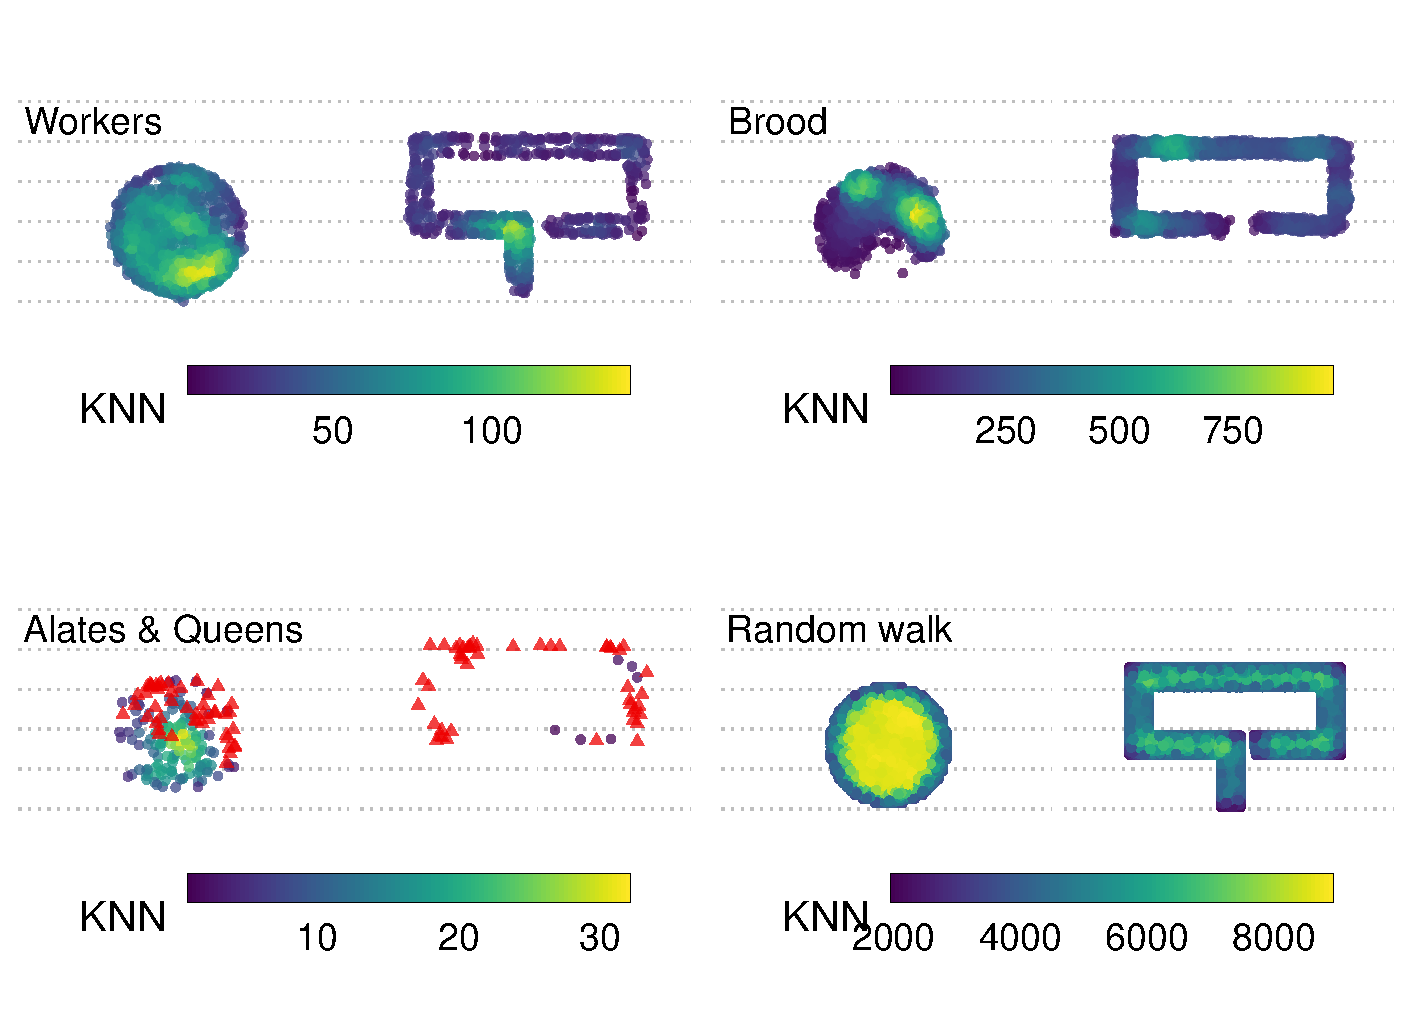
\includegraphics[width=0.9\linewidth,height=0.55\textheight]{/Users/gregchism/Library/Mobile Documents/com~apple~CloudDocs/Desktop/NestArchOrg/analysis/figures/Fig2} \end{flushleft}

\textbf{Figure 2}. Illustration of colony distribution in nests for one
example colony (no. 11). Shown are the distributions of workers
(top-left), brood and queens (top-right, queens are red triangles),
alates (bottom-left), and the low density Netlogo random walk simulated
workers (bottom-right). Distributions in circle nests are on the left
and the tube nest on the right. Each point is colored by the number of
k-nearest neighbors (KNN) within a radius that's standardized by the
data range (indicated by respective legends below each sub-figure).
Colony 11 was selected to illustrate all colony members since not all
colonies possess alates. The scatter plot grid for every colony, and
respective Netlogo simulation, can be found as Appendix, Figs. 12-31.

~

Workers and brood were found in nest sections closer to the entrance, in
relative terms, in the tube nest than in the circle nest (Workers:
\(\beta\) + SE = 0.003 + 0.001, t\textsubscript{3178} = 4.334, \emph{P}
\textless{} 0.001; Fig. 3, Appendix, Table A1), (Brood: \(\beta\) + SE =
-0.008 + 0.001, t\textsubscript{3170} = -6.122, \emph{P} \textless{}
0.001; Figs. 4a-b, Appendix, Table A2), but this was not seen in queens
(\(\beta\) + SE = -0.004 + 0.003, t\textsubscript{3178} = -1.403,
\emph{P} = 0.161, Figs. 4c-d, Appendix, Table A3) or alates (\(\beta\) +
SE = -0.001 + 0.004, t\textsubscript{448} = -0.150, \emph{P} = 0.881;
Fig. 4e, Appendix, Table A4). However, both queens (Appendix, Table A3)
and alates (Appendix, Table A4) were not evenly distributed in either
nest shape. All colony member distributions across nest sections were
therefore different between the two nest shapes, suggesting that
colonies have an occupation strategy different than evenly distributing
across nest space.

\begin{flushleft}\includegraphics[width=0.8\linewidth,height=0.6\textheight]{/Users/gregchism/Library/Mobile Documents/com~apple~CloudDocs/Desktop/NestArchOrg/analysis/figures/Fig3} \end{flushleft}

\textbf{Figure 3}. Workers tend to be clustered near the entrance in
both nest types, but this is more pronounced in the tube nest: shown
here are the worker (`Obsv', solid colors) and Netlogo simulated random
walk result (`RandWalk', white) proportions of workers in each nest
section of the tube (a, b; red) and circle (c, d; blue) nests (each
section has the same area across both nest types, but is scaled with
colony size). These figures also show the high (a, c) and low (b, d)
nest density treatment. Here, and in all following boxplots, boxes
represent first and third quartiles (75\% of the data), the bar within
boxes is the median, and whiskers are the data range. Sample size was
3192 worker proportions in nest sections across 20 colonies.

\begin{flushleft}\includegraphics[width=0.7\linewidth,height=0.95\textheight]{/Users/gregchism/Library/Mobile Documents/com~apple~CloudDocs/Desktop/NestArchOrg/analysis/figures/Fig3} \end{flushleft}

\textbf{Figure 4}. Brood and queens, but not alates, are generally found
further from the entrance than workers in both nest types shown here are
the difference in brood (a, b), queen (c, d) and alate (e) proportions
across tube (red) and circle (blue) nest sections. The brood and queen
densities are represented in both the high (a, c) and low (b, d) nest
density treatments. Note that here, and below, alates were only present
in the low nest density treatment. Sample sizes for colony members in
nest sections: brood = 3184, queen = 3192, alates = 456.

~

\emph{Brood in low nest density were more evenly distributed in each
nest shape}

Represented by a three-way interaction between nest shape, nest density,
and nest section, brood were distributed more evenly at the low density
treatment in both nest shapes, and they were found closer to the back of
the circle nest at high nest density when compared to the tube nest
shape (Brood: \(\beta\) + SE = 0.004 + 0.002, t\textsubscript{3170} =
2.513, \emph{P} = 0.012; Figs. 4a-b, Appendix, Table A2). In contrast,
there was no significant three-way interaction between nest shape,
density, and section in workers (\(\beta\) + SE = -0.002 + 0.001,
t\textsubscript{3178} = -1.695, \emph{P} = 0.090; Fig. 3, Appendix,
Table A1), or queens (\(\beta\) + SE = 0.001 + 0.004,
t\textsubscript{3178} = 0.308, \emph{P} = 0.758, Figs. 4c-d, Appendix,
Table A3). Therefore, brood care may be distributed across more nest
space in lower densities, but mobile colony members occupy nest space
similarly across densities.

~

\emph{No differences between colonies in overall colony member
distributions in nest sections}

In our models, 0.00\% of variation in the proportions of workers, brood,
queens, and alates in nest sections is explained by ColonyID (Appendix,
Tables A1-4).

~

\textbf{\emph{Distances from specific points in the nest}}

\emph{Nest shape affected colony member distance to the nest entrance}

Our tube nest design was long and narrow, thus allowing colony members
to be located at much further farther actual distances from the entrance
in the tube nest than was possible in the circle nest: (Workers:
Appendix, Figs. A8a-b, Table A5), (Brood: Appendix, Figs. A9a-b, Table
A6), (Queens: Appendix, Figs. A9c-d, Table A7), (Alates: Appendix, Figs.
A9e-f, Table A8). We further found that male alates were closer than
queen alates to the nest entrance in both nest shapes (Appendix, Fig.
A9f, Table A8). As they settled in the nest, workers (Appendix, Table
A5), brood (Appendix, Table A6), and queens (Appendix, Table A6) moved
closer to the nest entrance (Appendix, Tables A5-8), but alates moved
farther over time (Appendix, Table A8). These results suggest that
shorter distances to the entrance are an important factor in
\emph{Temnothorax rugatulus} nest occupation.

~

\emph{Nest shape affected mobile colony member distance to the brood
center}

All mobile colony members, i.e.~workers, queens, and alates, were also
farther from the brood center in the tube nest shape: (Workers:
\(\beta\) + SE = 0.103 + 0.002, t\textsubscript{26669.530} = 45.530,
\emph{P} \textless{} 0.001; Figs. 7a-b, Appendix, Table A9), (Queens:
\(\beta\) + SE = 0.090 + 0.011, t\textsubscript{1067.062} = 8.143,
\emph{P} \textless{} 0.001; Figs. 7c-d; Appendix, Table A10), (Alates:
\(\beta\) + SE = 0.211 + 0.018, t\textsubscript{2.895} = 11.672,
\emph{P} = 0.002; Fig. 7e, Appendix, Table A11). We also found that male
alates were found farther from the brood center than queen alates
(Appendix, Table A11). We lastly found that mobile colony member
distances to the brood center did not change over the course of the
experiment (Appendix, Tables A9-11). Therefore, nest shapes that
elongate nest space (e.g.~like our tube nest) likely force mobile colony
members to distances farther from the brood center.

\begin{flushleft}\includegraphics[width=0.7\linewidth,height=0.95\textheight]{/Users/gregchism/Library/Mobile Documents/com~apple~CloudDocs/Desktop/NestArchOrg/analysis/figures/Fig5} \end{flushleft}

\textbf{Figure 5}. Worker and queen distributions center near the center
of the brood distribution; but in the tube nest, the distances of both
from the brood center are much larger. The peak of alate distributions
is away from the brood center. Shown on the x-axis are the actual
distances from the brood center (see Methods), scaled only by setting
the farthest point of the tube nest as a distance of 1 (instead of
dividing the nest into sections as in Figs. 3-4). This implies that
distances given here are also scaled with colony size. Panels show
workers (a, b), queens (c, d), and alates (e, f). The difference between
male and female alates is shown in (f), denoted by letters A for females
and B for males. Differences in distributions are additionally shown
across high (a, c) and low (b, d) nest densities. Sample sizes for
colony member distances from the brood center: workers = 26733, queens =
1080, alates = 676.

~

\emph{Nest density increased worker and brood distance to the entrance
in each nest shape}

Workers and brood were found farther from the nest entrance in both nest
shapes at low nest density, but this was more pronounced in the tube
nest shape (Workers: Figs. 3a-b, Appendix, Figs. A8a-b, Table A5),
(Brood: Figs. 4a-b, Appendix, Figs. A9a-b, Table A6). In contrast, there
was no effect of nest density on queen distances from the entrance in
each nest (Queens: Figs. 4c-d, Appendix, Figs. A9c-d, Table A7). These
results may imply that at low density, colonies do not prioritize being
near the entrance, perhaps because of short travel times.

~

\emph{Nest density decreased worker distance to the brood center both
nest shapes}

We saw that workers were farther from the brood center in low nest
density, which was more pronounced in the tube nest (Workers: \(\beta\)
+ SE = 0.034 + 0.003, t\textsubscript{26709.876} = 11.769, \emph{P}
\textless{} 0.001; Figs. 5a-b, Appendix, Table A9), but queen distances
to the brood center were not different across density treatments
(Queens: \(\beta\) + SE = 0.001 + 0.013, t\textsubscript{1060.719} =
0.105, \emph{P} = 0.916; Figs. 5c-d; Appendix, Table A10). Queen
placement in nest shapes is likely more influenced by distance to the
brood center than the entrance, while workers are possibly more
influenced by distance to the nest entrance.

~

\emph{Small differences between colonies in distance relationships,
particularly in alates}

For proximity to the nest entrance, the model variation explained by
colony ID was 1.5\% for workers (Marginal R\textsuperscript{2+} = 0.337,
Conditional R\textsuperscript{2+} = 0.352, Appendix, Table A5), 4.8\%
for brood (Marginal R\textsuperscript{2+} = 0.439, Conditional
R\textsuperscript{2+} = 0.487, Appendix, Table A6), 7.2\% for queens
(Marginal R\textsuperscript{2+} = 0.492, Conditional
R\textsuperscript{2+} = 0.564, Appendix, Table A7), and 17.2\% for
alates (Marginal R\textsuperscript{2+} = 0.451, Conditional
R\textsuperscript{2+} = 0.623, Appendix, Table A8). Concerning proximity
to the brood center, the model variation explained by ColonyID was 2.2\%
for workers (Marginal R\textsuperscript{2+} = 0.279, Conditional
R\textsuperscript{2+} = 0.301, Appendix, Table A9), 8.6\% for queens
(Marginal R\textsuperscript{2+} = 0.249, Conditional
R\textsuperscript{2+} = 0.335, Appendix, Table A10), and 0.6\% for
alates (Marginal R\textsuperscript{2+} = 0.340, Conditional
R\textsuperscript{2+} = 0.346, Appendix, Table A11).

~

\textbf{\emph{Worker site fidelity}}

\emph{Scaled worker site fidelity was influenced by neither nest shape
nor nest density}

Nest shape did not influence worker spatial fidelity zone size as
measured in nest sections ( \(\beta\) + SE = -0.145 + 0.146,
t\textsubscript{378.727} = -0.994, \emph{P} = 0.321; Figs. 8a-b,
Appendix, Table A12) or occurrence zone size in this measurement
(\(\beta\) + SE = -0.080 + 0.214, t\textsubscript{378.858} = -0.372,
\emph{P} = 0.710; Figs. 8b-c, Appendix, Table A13), nor did nest density
(Fidelity zones: \(\beta\) + SE = -0.320 + 0.159,
t\textsubscript{14.107} = -2.010, \emph{P} = 0.064, Appendix, Tables
A12) (Occurrence zones: \(\beta\) + SE = 0.282 + 0.248,
t\textsubscript{19.358} = 1.137, \emph{P} = 0.270, Appendix, Tables
A13). Therefore, ant workers appear to be able to maintain the same site
fidelity regardless of nest shape.

\begin{flushleft}\includegraphics[width=0.7\linewidth,height=0.5\textheight]{/Users/gregchism/Library/Mobile Documents/com~apple~CloudDocs/Desktop/NestArchOrg/analysis/figures/Fig6} \end{flushleft}

\textbf{Figure 6}. Comparison of worker fidelity and occurrence zones
sizes (cm2) in the circle (blue) and tube (red) nests for both the high
(a, c) and low (b, d) nest density treatments. Fidelity zone sizes are
the same in each nest shape (\(\beta\) + SE = -0.022 + 0.044,
t\textsubscript{377.968} = -0.494, \emph{P} = 0.622, Appendix, Table
A14) and across density treatments (\(\beta\) + SE = 0.148 + 0.082,
t\textsubscript{19.161} = 1.799, \emph{P} = 0.088, Appendix, Table A14).
Occurrence zone sizes are the same in each nest shape (\(\beta\) + SE =
-0.023 + 0.071, t\textsubscript{366.580} = -0.324, \emph{P} = 0.746,
Appendix, Table A15) but are larger in lower nest density (\(\beta\) +
SE = 0.808 + 0.337, t\textsubscript{16.682} = 2.398, \emph{P} = 0.029,
Appendix, Table A15). Histograms represent the data distribution;
boxplots are the first and third quartiles where the black bar is the
median and the whiskers extend to the data range. Please see the methods
for details on how scaled worker fidelity and occurrence zone size
calculations, which here were multiplied by the total area of the nest
to achieve unscaled zone sizes. The sample size was 383 marked ants
across 19 colonies.

~

\emph{Worker identity explained some worker site fidelity variation}

The model variation explained (notably small) by the random effect
ColonyID was 4.6\% in fidelity zone sizes (marginal
R\textsuperscript{2+} = 0.022, conditional R\textsuperscript{2+} =
0.068, Appendix, Table A12) and 6.3\% in scaled occurrence zone sizes
(marginal R\textsuperscript{2+} = 0.015, conditional
R\textsuperscript{2+} = 0.078, Appendix, Table A13).

~

\begin{flushleft}\includegraphics[width=0.7\linewidth,height=0.5\textheight]{/Users/gregchism/Library/Mobile Documents/com~apple~CloudDocs/Desktop/NestArchOrg/analysis/figures/Fig7} \end{flushleft}

\textbf{Figure 7}. Relationship between true worker fidelity and
occurrence zones sizes (cm2) and colony size in the circle (blue) and
tube (red) nests for both the high (a, c) and low (b, d) nest density
treatments. Points are jittered on the x and y axis. Lines show
significant linear relationships, but note that the relationships in (a,
c) and (b, d) are not significantly different (Appendix, Tables A16-17).
The sample size was 383 marked ants across 19 colonies.

~

\textbf{\emph{Worker site fidelity and distances in the nest}}

\emph{No consistent relationship between worker site fidelity and
distance to the nest entrance}

We saw that both worker spatial fidelity and occurrence zones had
inconsistent relationships with that worker's distance to the nest
entrance both across nest shapes and nest densities (\(\beta\) + SE =
6.710 + 3.339, t\textsubscript{375} = 2.010, \emph{P} = 0.045; Appendix,
Figs. A10a-b, Table A18), (\(\beta\) + SE = -14.610 + 4.870,
t\textsubscript{374.994} = -3.000, \emph{P} = 0.003; Appendix, Figs.
A10c-d, Table A19) - e.g.~fidelity zones: the relationship in the circle
nest was positive in high density but negative in low density, both of
which were the opposite of the tube nest relationships in their
respective nest densities (Figs. Appendix, Figs. A10a-b, Table A18).
Therefore, we did not find a consistent relationship between worker site
fidelity and distance to the nest entrance.

~

\emph{Distance to the brood center did not influence spatial fidelity
zones}

There was no relationship between worker spatial fidelity zones and
distance from the brood center (\(\beta\) + SE = 1.517 + 4.715,
t\textsubscript{360.029} = 0.322, \emph{P} = 0.748; Figs. 8a-b,
Appendix, Table A20), but occurrence zones had an inconsistent
relationship both across nest shapes and nest densities (\(\beta\) + SE
= 18.951 + 6.889, t\textsubscript{374.920} = 2.751, \emph{P} = 0.006;
Figs. 8c-d, Appendix, Table A21). We therefore do not find that workers
in different areas of the nest have differently sized spatial fidelity
zones.

\begin{flushleft}\includegraphics[width=0.7\linewidth,height=0.5\textheight]{/Users/gregchism/Library/Mobile Documents/com~apple~CloudDocs/Desktop/NestArchOrg/analysis/figures/Fig8} \end{flushleft}

\textbf{Figure 8}. The relationship between scaled individual worker
fidelity (a, b) and occurrence (c, d) zone sizes (scaled relative to
total nest size, which was related to colony size) and average scaled
distance to the brood pile in the circle (blue circles, solid lines) and
tube (red triangles, dashed lines) nest shapes. Lines represent
significant linear relationships. These differences are additionally
compared across the high (a, c) and low (b, d) nest density treatments.
There were no significant differences in any scaled zone sizes across
nest shapes or density treatments (Appendix, Tables A20-21). The sample
size was 383 marked ants across 19 colonies.

~

\emph{Workers have spatial fidelity in relation to the brood center
across nest shapes}

Individual workers were found at different distances from the brood
center across all observations that they were identifiable (ANOVA:
F\textasciitilde380, 2328\textasciitilde{} = 4.180, \emph{P} \textless{}
0.001, Appendix, Table A22). We therefore can conclude that though
workers did not have consistent spatial fidelity zone sizes (Appendix,
Table A12), workers held repeatable spatial fidelity in their distances
from the brood center.

~

\emph{Small differences between colonies in the relationship between
worker site fidelity and nest distances}

In models of the relationship between worker site fidelity and distance
to the entrance, we saw that the variation explained by our random
effect (ColonyID) was 3.7\% for fidelity zone size (marginal R2 = 0.045,
conditional R2 = 0.082, Appendix, Table A18) and 6.2\% for occurrence
zone size (marginal R2 = 0.041, conditional R2 = 0.103, Appendix, Table
A19). In models of the relationship between worker site fidelity and
distance to the brood center, we saw that the variation explained by our
random effects was 3.1\% for fidelity zone size (marginal R2 = 0.036,
conditional R2 = 0.067, Appendix, Table A20) and 8.0\% for occurrence
zone size (marginal R2 = 0.038, conditional R2 = 0.118, Appendix, Table
A21).

\textbf{\emph{Random walk simulations}}

\emph{Empirical worker distributions differed from those predicted by a
random walk}

We saw that empirical and random walk simulated distributions were
different (Appendix, Tables A23-26). Specifically, simulated agents were
more evenly distributed, while real (observed) workers were found closer
to the nest entrance (NestSection2 * Nest * WorkerType: \(\beta\) + SE =
-0.002 + 0.000, t\textsubscript{35167} = -5.385, \emph{P} \textless{}
0.001; Fig. 3, Appendix, Table A24). The spatial distribution of ant
colonies in their nests is thus significantly different from the outcome
that would result from a random walk.

\emph{Empirical worker peak distributions differed from those predicted
by a random walk}

We saw that the nest section with the highest proportion of workers
(peak worker distribution) was closer to the entrance in the tube nest
than the circle nest, whereas simulated peaks were equally likely to be
in any nest section (NestSection2 * WorkerType * Nest: \(\beta\) + SE =
-0.133 + 0.041, z\textsubscript{35168} = -3.262, \emph{P} = 0.001;
Appendix, Fig. A11, Appendix, Table A25).

\textbf{Discussion}

Available nest shape influences the spatial organization of colonies in
the rock-dwelling ant \emph{Temnothorax rugatulus}. Overall, ants
preferred the areas in their nest that were closer to the entrance and
moved closer to the entrance over the 10 days of our measurements. But
in the tube-shaped nest, we found that workers, brood, queens, and
alates were on average located further from the nest entrance (Figs.
3-4, Appendix, Figs. A8-9) and further from the brood pile compared to
the circle nest (Fig. 5), presumably because the circle nest did not
allow such longer distances, but maybe also because of a lack of
available space closer to these points in the tube nest. Supporting this
second interpretation, workers, brood, and queens were found closer to
the nest entrance relative to the maximum available distance in that
nest type in the tube-shaped nest. None of these patterns are explained
by a null model of ants moving around randomly in the same nest shapes
(Fig. 3, Appendix, Figs. A8, A11). Nest shape alone could therefore
significantly impact the distances between individuals and biologically
relevant points in the nest, and thus how ants can interact with each
other and their nest space.

We found, however, that both worker spatial fidelity zone sizes and
overall area used by each worker (`occurrence zone' size) were not
affected by nest shape, either when measured in absolute area or
relative to total nest size (Figs. 6, 8). We also did not find a
consistent relationship of these zone sizes with location in the nest
(e.g.~distance to the brood pile, Fig. 8). This is different from what
has been demonstrated previously in both \emph{Temnothorax unifasciatus}
and the bumble bee \emph{Bombus impatiens}; in both species, workers
further from the nest center (brood pile) had larger spatial fidelity
zones (Sendova-Franks and Franks 1995; Jandt and Dornhaus 2009).
However, our result is consistent with earlier studies on our species
\emph{T. rugatulus} which showed that while inactive workers tended to
both have small spatial fidelity zones and remain near the nest center
while inactive, this was not the case when including these workers'
active phases (Charbonneau et al., 2017). We however found that
individual workers held spatial fidelity over time in relation to
distance from the brood center, despite no consistent trends. The site
fidelity of social insect workers in the nest may relate to task
specialization, as certain tasks are more likely to be performed in
specific nest sections (Sendova-Franks and Franks 1995); smaller
fidelity zones thus may be connected to and allow for more specialized
workers. Given that workers are more crowded in the tube-shaped nest in
our experiment, the lack of a consistent effect on worker spatial
fidelity zones may suggest that workers actively regulate their zone
size even against constraints imposed by nest shape, to maintain a
desired association between workers and their tasks. This bears further
investigation.

Our study confirms that the spatial distribution of colony members in
ant nests is not identical to one that would be produced by `random
movement'. We do not propose that it is realistic that ants move
randomly; rather, we believe this is an appropriate null hypothesis to
clarify whether the outcome of movement is in fact different from one in
which individual actions do not add up to a non-random trend to
accumulate in particular areas. In other studies, the outcome of ant
movement has sometimes been indistinguishable from similar null
hypotheses of randomness (e.g.~worker sorting: Sendova-Franks and Van
Lent 2002; interactions between potential and returning foragers:
Davidson and Gordon 2017). Additionally, movement in the nest from one
ant \emph{T. albipennis} can be predicted by movement from another, and
faster movement occurs when more ants are in motion (Gallotti and
Chialvo 2018). Outside of the nest, random movement that is reinforced
by trail pheromones explains ant coordination along specific trails to
and from food sources and the nest (Ma et al., 2013; Chang et al.,
2021). The non-random nest occupation of our \emph{T. rugatulus}
colonies therefore demonstrates not only that individual ants' movement
is not random, but that in aggregate, individual movement rules are such
that they bias worker movement to produce clustering and heterogeneity
in distribution at the colony level, and that the effects of nest shape
we find here cannot be produced by passive effects of geometry on random
movement.

The total area available in an enclosed ant nest will determine worker
density. Both nest area and worker density in the nest have previously
been demonstrated to be important in ants, and our results support this.
Nest area is an important consideration for nest site selection in
\emph{Temnothorax} ants (Pratt and Pierce 2001; Mitrus 2015), where
workers measure the size of prospective nests (Pratt 2005). Crowded
nests can significantly increase worker energy expenditure in \emph{T.
rugatulus} colonies (Cao and Dornhaus 2008), while also both increasing
foraging and scouting rates and inducing polydomy (Cao 2013). The
consequences of nest density to ant colonies, such as traffic jammed
panicked nest evacuation, can be mediated by small structural features
at the nest entrance (Burd et al., 2010; Shiwakoti et al., 2014; Wang
and Song 2016). Ants may even adaptively regulate contact rate with each
other, as a part of strategies for task allocation and information
exchange (Pacala et al., 1996; Pinter-Wollman et al., 2012;
Pinter-Wollman et al., 2013; Lehue et al., 2020b). Contact rate may also
be used to estimate colony or group size (Gordon et al., 1992; Pratt
2005; Dornhaus and Franks 2006). In our study here, we compared colonies
at two different worker densities, but also found that local density in
nests is heterogeneous and may be driven by overall nest shape and thus
access to all parts of the nest. We saw that colony members spread out
more in both nest shapes at low worker density, but this effect was more
pronounced in the tube nest shape; in addition, we saw that constraints
of space led to higher local density near the entrance in the tube nest
(e.g.~see Figs. 3-4). Our study did not address whether the spatial
distribution of colony members in their nests is a passive effect of
particular cavity shapes and densities, or a result of adaptive,
flexible individual strategies used by \emph{Temnothorax} ants in
response to the particular nest spaces encountered. \emph{Temnothorax}
ants, in nature, can also modify their nest spaces by adding internal
stone walls to the cavity their nest inhabits (Franks et al., 1992;
Franks and Deneubourg 1997; Aleksiev et al., 2007a; Aleksiev et al.,
2007b; Aleksiev et al., 2007c; DiRienzo and Dornhaus 2017). The purpose
of such nest modifications is not well studied, but it is a possibility
that these ants actively modify either the available area or the shape
of their nest space. Future work may reveal more about how these spatial
distributions affect colony performance, and thus spatial properties of
both nest cavities and colony distribution matter most to colonies.

Overall, we found that nest shape affected how ants of the species
\emph{T. rugatulus} occupied their nests, and therefore traits of nest
cavities available in the ants' environment may affect the behaviour of
the colonies inhabiting them. Nest geometry may affect the accessibility
of the nest entrance and center of the brood pile, and it may affect
ant-ant interactions through heterogeneity in worker density in the
nest. On the other hand, we found that at least one important
characteristic of the distribution of ant workers in their nests, namely
the `spatial fidelity zone size' for ant workers, appears resilient to
such changes in nest shape. It is therefore possible that such
resilience is the result of evolved strategies by ant workers to deal
with such variability in nest geometry. We argue that nest shape and
worker density need to be considered when studying topics such as worker
site fidelity, task specialization, overall nest space usage, and nest
site selection in ant colonies. Both the approach and results of our
study could possibly be extended to other social animal architects, such
naked mole rats, social crabs, and social weaver birds, providing
insights into how the structural components of their built architectures
(i.e.~burrows, nests) can influence occupant behaviours such as kinship
and division of labor.

\hypertarget{acknowledgements}{%
\section{Acknowledgements}\label{acknowledgements}}

The authors thank Colin Lynch, Victor (Blue) Paat, Michaela Stearman,
Lovina Hadley, Wiley Faron, Kerry Marquardt and Mariya Belishka for
their integral work in collecting the data for this study. The authors
acknowledge funding from the National Science Foundation awarded to AD
(grants no. IOS-3014230 and ABI-3019760) and to GC (grant no.
IOS-3014230).

\hypertarget{references}{%
\section{References}\label{references}}

~~ Allaire, J. (2012). \emph{RStudio: integrated development environment
for R}. Boston, MA, 770(394), 165-171. URL: http://www.rstudio.com/

~~ Aleksiev, A. S., Longdon, B., Christmas, M. J., Sendova-Franks, A.
B., and Franks, N. R. (2007a). Individual choice of building material
for nest construction by worker ants and the collective outcome for
their colony. \emph{Animal Behaviour}, \emph{74}(3), 559-566.
https://doi.org/10.1016/j.anbehav.2006.12.019

~~ Aleksiev, A. S., Sendova-Franks, A. B., and Franks, N. R. (2007b).
Nest `moulting' in the ant \emph{Temnothorax albipennis}. \emph{Animal
Behaviour}, \emph{74}(3), 567-575.
https://doi.org/10.1016/j.anbehav.2006.12.023

~~ Aleksiev, A. S., Sendova-Franks, A. B., and Franks, N. R. (2007c).
The selection of building material for wall construction by ants.
\emph{Animal Behaviour}, \emph{73}(5), 779-788.
https://doi.org/10.1016/j.anbehav.2006.06.014

~~ Anderson, T. W. (1962). On the Distribution of the Two-Sample
Cramer-von Mises Criterion. \emph{Ann. Math. Statist.} 33(3) 1148 -
1159. https://doi.org/10.1214/aoms/1177704477

~~ Bartoń, K. (2020). \emph{MuMIn: multi-model inference. R package
version 1.43. 17}. Vienna, Austria: The Comprehensive R Archive Network
(CRAN) https://CRAN.R-project.org/package=MuMIn ~~ Bates, D., Mächler,
M., Bolker, B., and Walker, S. (2014). Fitting linear mixed-effects
models using lme4. \emph{arXiv} preprint arXiv:1406.5823.
https://doi.org/10.18637/jss.v067.i01

~~ Benjamini, Y., and Hochberg, Y. (1995). Controlling the false
discovery rate: a practical and powerful approach to multiple testing.
\emph{Journal of the Royal Statistical Society: Series B
(Methodological)}, \emph{57}(1), 289-300.
https://doi.org/10.1111/j.2517-6161.1995.tb02031.x

~~ Bengston, S. E., and Dornhaus, A. (2014). Be meek or be bold? A
colony-level behavioural syndrome in ants. \emph{Proceedings of the
Royal Society B: Biological Sciences}, \emph{281}(1791), 20140518.
https://doi.org/10.1098/rspb.2014.0518

~~ Bengston, S. E., and Dornhaus, A. (2015). Latitudinal variation in
behaviors linked to risk tolerance is driven by nest-site competition
and spatial distribution in the ant \emph{Temnothorax rugatulus}.
\emph{Behavioral Ecology and Sociobiology}, 69(8), 1265-1274.
https://doi.org/10.1007/s00265-015-1939-4

~~ Bengston, S. E., Shin, M., and Dornhaus, A. (2017). Life-history
strategy and behavioral type: risk‐tolerance reflects growth rate and
energy allocation in ant colonies. \emph{Oikos}, \emph{126}(4), 556-564.
https://doi.org/10.1111/oik.03527

~~ Burd, M., Shiwakoti, N., Sarvi, M., and Rose, G. (2010). Nest
architecture and traffic flow: large potential effects from small
structural features. \emph{Ecological Entomology}, \emph{35}(4),
464-468. https://doi.org/10.1111/j.1365-2311.2010.01202.x

~~ Cao, T. T., and Dornhaus, A. (2008). Ants under crowded conditions
consume more energy. \emph{Biology Letters}, \emph{4}(6), 613-615.
https://doi.org/10.1098/rsbl.2008.0381

~~ Cao, T. T. (2013). High social density increases foraging and
scouting rates and induces polydomy in \emph{Temnothorax} ants.
\emph{Behavioral Ecology and Sociobiology}, \emph{67}(11), 1799-1807.
https://doi.org/10.1007/s00265-013-1587-5

~~ Chang, J., Powell, S., Robinson, E. J., and Donaldson-Matasci, M. C.
(2021). Nest choice in arboreal ants is an emergent consequence of
network creation under spatial constraints. \emph{Swarm Intelligence},
\emph{15}(1), 7-30. https://doi.org/10.1007/s11721-021-00187-5

~~ Charbonneau, D., and Dornhaus, A. (2015). Workers `specialized' on
inactivity: behavioral consistency of inactive workers and their role in
task allocation. \emph{Behavioral Ecology and Sociobiology},
\emph{69}(9), 1459-1472. https://doi.org/10.1007/s00265-015-1958-1

~~ Charbonneau, D., Hillis, N., and Dornhaus, A. (2015). `Lazy' in
nature: ant colony time budgets show high `inactivity' in the field as
well as in the lab. \emph{Insectes Sociaux}, 62(1), 31-35.
https://doi.org/10.1007/s00040-014-0370-6

~~ Charbonneau, D., Poff, C., Nguyen, H., Shin, M. C., Kierstead, K.,
and Dornhaus, A. (2017). Who are the ``lazy'' ants? The function of
inactivity in social insects and a possible role of constraint: inactive
ants are corpulent and may be young and/or selfish. \emph{Integrative
and Comparative Biology}, \emph{57}(3), 649-667.
https://doi.org/10.1093/icb/icx029

~~ Charbonneau, D., Sasaki, T., and Dornhaus, A. (2017). Who needs
`lazy' workers? Inactive workers act as a `reserve' labor force
replacing active workers, but inactive workers are not replaced when
they are removed. \emph{PLoS ONE}, 12(9), e0184074.
https://doi.org/10.1371/journal.pone.0184074

~~ Davidson, J. D., and Gordon, D. M. (2017). Spatial organization and
interactions of harvester ants during foraging activity. Journal of The
Royal Society Interface, 14(135), 20170413.
https://doi.org/10.1098/rsif.2017.0413

~~ DiRienzo, N., and Dornhaus, A. (2017). Temnothorax rugatulus ant
colonies consistently vary in nest structure across time and context.
PLoS One, 12(6), e0177598. https://doi.org/10.1371/journal.pone.0177598

~~ Dornhaus, A., Franks, N. R., Hawkins, R. M., and Shere, H. N. S.
(2004). Ants move to improve: colonies of Leptothorax albipennis
emigrate whenever they find a superior nest site. Animal Behaviour,
67(5), 959-963. https://doi.org/10.1016/j.anbehav.2003.09.004

~~ Dornhaus, A., and Franks, N. R. (2006). Colony size affects
collective decision-making in the ant Temnothorax albipennis. Insectes
Sociaux, 53(4), 420-427. https://doi.org/10.1007/s00040-006-0887-4

~~ Dowd, C. (2020). A New ECDF Two-Sample Test Statistic. arXiv preprint
arXiv:2007.01360. URL: https://arxiv.org/abs/2007.01360

~~ Faulkes, C. G., and Bennett, N. C. (2001). Family values: group
dynamics and social control of reproduction in African mole-rats. Trends
in Ecology and Evolution, 16(4), 184-190.
https://doi.org/10.1016/S0169-5347(01)02116-4

~~ Franks, N. R., Wilby, A., Silverman, B. W., and Tofts, C. (1992).
Self-organizing nest construction in ants: sophisticated building by
blind bulldozing. Animal Behaviour, 44, 357-375.
https://doi.org/10.1016/0003-3472(92)90041-7

~~ Franks, N. R., and Deneubourg, J. L. (1997). Self-organizing nest
construction in ants: individual worker behaviour and the nest's
dynamics. Animal Behaviour, 54(4), 779-796.
https://doi.org/10.1016/0003-3472(92)90041-7

~~ Franks, N. R., Pratt, S. C., Mallon, E. B., Britton, N. F., and
Sumpter, D. J. (2002). Information flow, opinion polling and collective
intelligence in house--hunting social insects. Philosophical
Transactions of the Royal Society of London B: Biological Sciences,
357(1427), 1567-1583. https://doi.org/10.1098/rstb.2002.1066

~~ Gallotti, R., and Chialvo, D. R. (2018). How ants move: individual
and collective scaling properties. Journal of The Royal Society
Interface, 15(143), 20180223. https://doi.org/10.1098/rsif.2018.0223

~~ Gordon, D. M. (1992). Nest relocation in harvester ants. Annals of
the Entomological Society of America, 85(1), 44-47.
https://doi.org/10.1093/aesa/85.1.44

~~ Heyman, Y., Shental, N., Brandis, A., Hefetz, A., and Feinerman, O.
(2017). Ants regulate colony spatial organization using multiple
chemical road-signs. Nature Communications, 8(1), 1-11.
https://doi.org/10.1038/ncomms15414

~~ Jandt, J. M., and Dornhaus, A. (2009). Spatial organization and
division of labour in the bumblebee Bombus impatiens. Animal Behaviour,
77(3), 641-651. https://doi.org/10.1007/s00265-011-1244-9

~~ Kuznetsova, A., Brockhoff, P. B., and Christensen, R. H. (2017).
lmerTest package: tests in linear mixed effects models. Journal of
Statistical Software, 82(1), 1-26. https://doi.org/10.18637/jss.v082.i13

~~ Laidre, M. E., Wellborn, G. A., and Thiel, M. (2018). Evolutionary
ecology of burrow construction and social life (pp.~279-301). New York,
NY: Oxford University Press.

~~ Laidre, M. E. (2019). Architectural modification of shells by
terrestrial hermit crabs alters social dynamics in later generations.
Ecology, 100(9), e02767. https://doi.org/10.1002/ecy.2767

~~ Lehue, M., and Detrain, C. (2019). What's going on at the entrance? A
characterisation of the social interface in ant nests. Behavioural
Processes, 160, 42-50. https://doi.org/10.1016/j.beproc.2018.12.006

~~ Lehue, M., and Detrain, C. (2020). Foraging through multiple nest
holes: An impediment to collective decision-making in ants. PLoS One,
15(7), e0234526. https://doi.org/10.1371/journal.pone.0234526

~~ Lehue, M., Collignon, B., and Detrain, C. (2020a). Multiple nest
entrances alter foraging and information transfer in ants. Royal Society
Open Science, 7(2), 191330. https://doi.org/10.1098/rsos.191330

~~ Lehue, M., Detrain, C., and Collignon, B. (2020b). Nest entrances,
spatial fidelity, and foraging patterns in the red ant Myrmica rubra: a
field and theoretical study. Insects, 11(5), 317.
https://doi.org/10.3390/insects11050317

~~ Leitner, N., and Dornhaus, A. (2019). Dynamic task allocation: how
and why do social insect workers take on new tasks?. Animal Behaviour,
158, 47-63. https://doi.org/10.1016/j.anbehav.2019.09.021

~~ Ma, Q., Johansson, A., Tero, A., Nakagaki, T., and Sumpter, D. J.
(2013). Current-reinforced random walks for constructing transport
networks. Journal of the Royal Society Interface, 10(80), 20120864.

~~ Mitrus, S. (2015). The cavity-nest ant Temnothorax crassispinus
prefers larger nests. Insectes Sociaux, 62(1), 43-49.
https://doi.org/10.1007/s00040-014-0372-4

~~ Pacala, S. W., Gordon, D. M., and Godfray, H. C. J. (1996). Effects
of social group size on information transfer and task allocation.
\emph{Evolutionary Ecology}, \emph{10}(2), 127-165.
https://doi.org/10.1007/BF01241782

~~ Pinter-Wollman, N., Hubler, J., Holley, J. A., Franks, N. R., and
Dornhaus, A. (2012). How is activity distributed among and within tasks
in \emph{Temnothorax} ants?. \emph{Behavioral Ecology and Sociobiology},
\emph{66}(10), 1407-1420.

~~ Pinter-Wollman, N., Bala, A., Merrell, A., Queirolo, J., Stumpe, M.
C., Holmes, S., and Gordon, D. M. (2013). Harvester ants use
interactions to regulate forager activation and availability.
\emph{Animal Behaviour}, \emph{86}(1), 197-207.
https://doi.org/10.1007/s00265-012-1396-2

~~ Pinter-Wollman, N. (2015). Nest architecture architectures the
collective behaviour of harvester ants. \emph{Biology Letters},
\emph{11}(10), 20150695. https://doi.org/10.1098/rsbl.2015.0695

~~ Powell, S. (2008). Ecological specialization and the evolution of a
specialized caste in \emph{Cephalotes} ants. \emph{Functional Ecology},
\emph{22}(5), 902-911. https://doi.org/10.1111/j.1365-2435.2008.01436.x

~~ Pratt, S. C., and Pierce, N. E. (2001). The cavity-dwelling ant
\emph{Leptothorax curvispinosus} uses nest geometry to discriminate
between potential homes. \emph{Animal Behaviour}, \emph{62}(2),
281--287. https://doi.org/10.1006/anbe.2001.1777

~~ Pratt, S. C. (2005). Quorum sensing by encounter rates in the ant
\emph{Temnothorax albipennis}. \emph{Behavioral Ecology}, \emph{16}(2),
488-496. https://doi.org/10.1093/beheco/ari020

~~ Prebus, M. (2017). Insights into the evolution, biogeography and
natural history of the acorn ants, genus \emph{Temnothorax} Mayr
(hymenoptera: Formicidae). \emph{BMC Evolutionary Biology},
\emph{17}(1), 1-22. https://doi.org/10.1186/s12862-017-1095-8

~~ R Core Team (2017). \emph{R: A language and environment for
statistical computing}. R Foundation for Statistical Computing, Vienna,
Austria. URL https://www.R-project.org/.

~~ Robinson, E. J., Feinerman, O., and Franks, N. R. (2009). Flexible
task allocation and the organization of work in ants. \emph{Proceedings
of the Royal Society B: Biological Sciences}, 276(1677), 4373-4380.
https://doi.org/10.1098/rspb.2009.1244

~~ Sasaki, T., and Pratt, S. C. (2013). Ants learn to rely on more
informative attributes during decision-making. \emph{Biology Letters},
\emph{9}(6), 20130667. https://doi.org/10.1098/rsbl.2013.0667

~~ Sasaki, T., Colling, B., Sonnenschein, A., Boggess, M. M., and Pratt,
S. C. (2015). Flexibility of collective decision making during house
hunting in \emph{Temnothorax} ants. \emph{Behavioral Ecology and
Sociobiology}, \emph{69}(5), 707-714.
https://doi.org/10.1093/beheco/arr007

~~ Schindelin, J., Arganda-Carreras, I., Frise, E., Kaynig, V., Longair,
M., Pietzsch, T., \ldots{} and Tinevez, J. Y. (2012). Fiji: an
open-source platform for biological-image analysis. \emph{Nature
methods}, \emph{9}(7), 676. https://doi.org/10.1038/nmeth.2019

~~ Sendova-Franks, A. B., and Franks, N. R. (1994). Social resilience in
individual worker ants and its role in division of labour.
\emph{Proceedings of the Royal Society of London. Series B: Biological
Sciences}, \emph{256}(1347), 305-309.
https://doi.org/10.1098/rspb.1994.0085

~~ Sendova-Franks, A. B., and Franks, N. R. (1995). Spatial
relationships within nests of the ant \emph{Leptothorax unifasciatus}
(Latr.) and their implications for the division of labour. \emph{Animal
Behaviour}, \emph{50}(1), 121-136.
https://doi.org/10.1006/anbe.1995.0226

~~ Sendova-Franks, A. B., and Franks, N. R. (1999). Self-assembly,
self-organization and division of labour. \emph{Philosophical
Transactions of the Royal Society of London B: Biological Sciences},
\emph{354}(1388), 1395-1405. https://doi.org/10.1098/rstb.1999.0487

~~ Sendova-Franks, A. B., and Van Lent, J. (2002). Random walk models of
worker sorting in ant colonies. \emph{Journal of Theoretical Biology},
\emph{217}(2), 255-274. https://doi.org/10.1006/jtbi.2002.3011

~~ Shiwakoti, N., Sarvi, M., and Burd, M. (2014). Using non-human
biological entities to understand pedestrian crowd behaviour under
emergency conditions. \emph{Safety Science}, \emph{66}, 1-8.
https://doi.org/10.1016/j.ssci.2014.01.010

~~ Thomas, M. L. (2002). Nest site selection and longevity in the
ponerine ant \emph{Rhytidoponera metallica} (Hymenoptera, Formicidae).
\emph{Insectes Sociaux}, \emph{49}(2), 147-152.
https://doi.org/10.1007/s00040-002-8294-y

~~ Tofts, C., and Franks, N. R. (1992). Doing the right thing: ants,
honeybees and naked mole-rats. \emph{Trends in Ecology and Evolution},
\emph{7}(10), 346-349. https://doi.org/10.1016/0169-5347(92)90128-X

~~ Tschinkel, W. R. (1999). Sociometry and sociogenesis of colonies of
the harvester ant, \emph{Pogonomyrmex badius}: distribution of workers,
brood and seeds within the nest in relation to colony size and season.
\emph{Ecological Entomology}, 24(2), 222-237.
https://doi.org/10.1673/2006\_06\_32.1

~~ Tschinkel, W. R. (2005). The nest architecture of the ant, Camponotus
socius. \emph{Journal of Insect Science}, \emph{5}(1).
https://doi.org/10.1093/jis/5.1.9

~~ Vaes, O., Perna, A., and Detrain, C. (2020). The effect of nest
topology on spatial organization and recruitment in the red ant
\emph{Myrmica rubra}. \emph{The Science of Nature}, \emph{107}, 1-14.
https://doi.org/10.1007/s00114-020-01675-0

~~ van Dijk, R. E., Covas, R., Doutrelant, C., Spottiswoode, C. N., and
Hatchwell, B. J. (2015). Fine-scale genetic structure reflects
sex-specific dispersal strategies in a population of sociable weavers (
\emph{Philetairus socius} ). \emph{Molecular Ecology}, \emph{24}(16),
4296-4311. https://doi.org/10.1111/mec.13308

~~ Varoudis, T., Swenson, A. G., Kirkton, S. D., and Waters, J. S.
(2018). Exploring nest structures of acorn dwelling ants with X-ray
microtomography and surface-based three-dimensional visibility graph
analysis. \emph{Philosophical Transactions of the Royal Society B:
Biological Sciences}, \emph{373}(1753), 20170237.
https://doi.org/10.1098/rstb.2017.0237

~~ Visscher, P. K. (2007). Group decision making in nest-site selection
among social insects. \emph{Annual Review of Entomology}, \emph{52},
255-275. https://doi.org/10.1146/annurev.ento.51.110104.151025

~~ Wang, S., and Song, W. (2016). Experimental study of ant movement in
a straight passageway under stress conditions. \emph{Journal of Insect
Behavior}, \emph{29}(6), 735-743.
https://doi.org/10.1007/s10905-016-9593-x

~~ Wickham, H., Averick, M., Bryan, J., Chang, W., McGowan, L. D. A.,
François, R., \ldots{} and Yutani, H. (2019). Welcome to the Tidyverse.
\emph{Journal of Open Source Software}, \emph{4}(43), 1686.
https://doi.org/10.21105/joss.01686

~~ Wilensky, U. (1999). \emph{NetLogo}.
http://ccl.northwestern.edu/netlogo/. Center for Connected Learning and
Computer-Based Modeling, Northwestern University, Evanston, IL.

~~ Wilson, E. O. (1992). The effects of complex social life on evolution
and biodiversity. \emph{Oikos}, 13-18. https://doi.org/10.2307/3545511

~~ Wilson, E. O., and Kinne, O. (1990). \emph{Success and dominance in
ecosystems: the case of the social insects} (Vol. 2, pp.~I-XXI).
Oldendorf/Luhe: Ecology Institute.

Appendix

\textbf{Table A1}. Proportions of workers in each nest section related
to nest shape and physical properties. Here and below: Sections
(NestSect) begin at the nest entrance (1) and complete at the back of
the nest (8) and is a quadratic term. Density is the amount of area
allocated for each worker (high = 0.033 cm2, low = 0.066 cm2 x 2), Day
is the observation day along the experimental timeline. Corner is the
presence of corners in the nest section. The random effect ColonyID is
colony identification. Asterisks denote interactions, and bold P values
indicate significance. Linear mixed effects model: PropWorker
\textasciitilde{} poly(NestSect, degree = 2, raw = TRUE) * Nest *
Density + Day + Corner + (1 \textbar{} ColonyID)

\textbf{Table A2}. Proportions of brood in each nest section related to
nest shape and physical properties. Linear mixed effects: PropBrood
\textasciitilde{} poly(NestSect, degree = 2, raw = TRUE) * Nest *
Density + Day + Corner + (1 \textbar{} ColonyID)

\textbf{Table A3}. Proportions of queens in each nest section related to
nest shape and physical properties. Linear mixed effects: PropQueens
\textasciitilde{} poly(NestSect, degree = 2, raw = TRUE) * Nest *
Density + Day + Corner + (1 \textbar{} ColonyID)

\textbf{Table A4}. Proportions of alates in each nest section related to
nest shape and physical properties. Linear mixed effects: PropAlates
\textasciitilde{} poly(NestSect, degree = 2, raw = TRUE) * Nest + Day +
Corner + (1 \textbar{} ColonyID)

\textbf{Table A5}. Relationships between workers scaled distance to the
nest entrance and nest shape and physical properties. Distance to the
entrance is scaled such that 1 is the back of the tube nest shape.
Linear mixed effects: ScaledDist \textasciitilde{} Nest * Density + Day
+ Corner + (1 \textbar{} ColonyID)

\textbf{Table A6}. Relationships between brood scaled distance to the
nest entrance and nest shape and physical properties. Linear mixed
effects: ScaledDist \textasciitilde{} Nest * Density + Day + Corner + (1
\textbar{} ColonyID)

\textbf{Table A7}. Relationships between queens scaled distance to the
nest entrance and nest shape and physical properties. Linear mixed
effects: ScaledDist \textasciitilde{} Nest * Density + Day + Corner + (1
\textbar{} ColonyID)

\textbf{Table A8}. Relationships between workers scaled distance to the
nest entrance and nest shape, nest physical properties, and alate sex.
Sex is male or female alates, and ratio is the proportion of male alates
over all alate types in the observation. Linear mixed effects:
ScaledDist \textasciitilde{} Nest + Sex + Ratio + Day + Corner + (1
\textbar{} ColonyID)

\textbf{Table A9}. Relationships between workers scaled distance to the
brood center and nest shape and physical properties. The brood center is
a colony's brood center in each observation. Distance to the brood
center is the absolute value of the difference between the scaled
distances of the brood center from each worker to the entrance and is
scaled such that 1 is the back of the tube nest. Linear mixed effects:
ToBrood \textasciitilde{} Nest * Density + Day + Corner + (1 \textbar{}
ColonyID) Table A10. Relationships between queen scaled distance to the
brood center and nest shape and physical properties. Linear mixed
effects: ToBrood \textasciitilde{} Nest * Density + Day + Corner + (1
\textbar{} ColonyID)

\textbf{Table A11}. Relationships between alate scaled distance to the
brood center and nest shape and physical properties. Linear mixed
effects: ToBrood \textasciitilde{} Nest + Sex + Ratio + Day + Corner +
(1 \textbar{} ColonyID)

\textbf{Table A12}. The relationship between worker spatial fidelity
zone size and nest shape. Fidelity zone size is the summation of all
zones that a worker was found in (zones must have at least 7
observations and 15\% of total observations), with twenty-four total
possible zones. Linear mixed effects: SFZ \textasciitilde{} Nest *
Density + (1 \textbar{} ColonyID)

\textbf{Table A13}. The relationship between worker occurrence zone size
and nest shape. Occurrence zone size is the ratio between the summation
of all zones that a worker was found in (zones must have at least 7
observations), and twenty-four (total possible zones). Linear mixed
effects: Occur \textasciitilde{} Nest * Density + (1 \textbar{}
ColonyID)

\textbf{Table A14}. The relationship between true worker spatial
fidelity zone size (cm2) and nest shape. Here and below the ratio
between the total number of occupied zones with \textgreater15\%
observations (fidelity zone size) and the twenty-four possible zones is
multiplied by nest area to produce true fidelity zone size. Linear mixed
effects: SFZ\_Area \textasciitilde{} Nest * Density + (1 \textbar{}
ColonyID)

\textbf{Table A15}. The relationship between true worker occurrence zone
size (cm2) and nest shape. Here and below the ratio between the total
number of occupied zones (occurrence zone size) and the twenty-four
possible zones is multiplied by nest area to produce true occurrence
zone size. Linear mixed effects: Occur\_Area \textasciitilde{} Nest *
Density + (1 \textbar{} ColonyID)

\textbf{Table A16}. The relationship between true worker spatial
fidelity zone size (cm2) and colony size (worker.number). Linear mixed
effects: SFZ\_Area \textasciitilde{} Number.workers * Nest * Density +
(1 \textbar{} ColonyID)

\textbf{Table A17}. The relationship between true worker occurrence zone
size (cm2) and colony size (worker.number). Linear mixed effects:
Occur\_Area \textasciitilde{} Number.workers * Nest * Density + (1
\textbar{} ColonyID)

\textbf{Table A18}. The relationship between a worker's spatial fidelity
zone size and average scaled distance to the nest entrance across nest
shapes. Linear mixed effects: SFZ \textasciitilde{} MeanScaledDist *
Nest * Density + (1 \textbar{} ColonyID)

\textbf{Table A19}. The relationship between a worker's occurrence zone
size and average scaled distance to the nest entrance across nest
shapes. Linear mixed effects: Occur \textasciitilde{} MeanScaledDist *
Nest * Density + (1 \textbar{} ColonyID)

\textbf{Table A20}. The relationship between a worker's spatial fidelity
zone size and average scaled distance to the brood center across nest
shapes. Linear mixed effects: SFZ \textasciitilde{} MeanToBrood * Nest *
Density + (1 \textbar{} ColonyID)

\textbf{Table A21}. The relationship between a worker's occurrence zone
size and average scaled distance to the brood center across nest shapes.
Linear mixed effects: Occur \textasciitilde{} MeanToBrood * Nest *
Density + (1 \textbar{} ColonyID)

\textbf{Table A22}. Individual worker (marked) fidelity in relation to
distance from the brood center across all observations. AntIDColNest is
each identifiable ant in the study. ANOVA: ToBrood \textasciitilde{}
Nest * Density + AntIDColNest

\textbf{Table A23}. Distribution comparisons between the worker and
Netlogo random walk simulation results. Two-sample Cramér-von Mises's
test statistics were calculated through 2000 random resample bootstraps
of the worker and simulated distributions, from which the P value was
derived. False Discovery Rates inherent to multiple comparisons were
corrected using the Benjamini-Hochberg method.

\textbf{Table A24}. The relationship between proportions of worker and
Netlogo random walk simulated results in each nest section and nest
shape and physical properties. WorkerType is whether the observation was
a worker or Netlogo random walk simulated result. Linear regression:
PropWorker \textasciitilde{} poly(NestSect, degree = 2, raw = TRUE) *
Nest * WorkerType * Density + Corner

\textbf{Table A25}. The maximum worker and Netlogo random walk simulated
result proportions in each nest section. Nest sections with the max
worker or simulated result proportion in each observation were assigned
a 1, where the other sections are 0. Logistic regression: MaxNestSect
\textasciitilde{} NestSect * WorkerType * Nest * Density, family =
Binomial

\textbf{Table A26}. Relationships between worker and Netlogo random walk
simulated result scaled distance to the nest entrance and nest shape and
physical properties. Linear regression: ScaledDist \textasciitilde{}
Nest * WorkerType + Density + Corner

\textbf{Figure A1}. The reference photo used to determine the nest area
allocated to each worker in a colony. The colony contains 248
individuals, determined with the image analysis software Fiji. The
internal area is approximately 4.11mm2, producing 0.017 mm2 for each
worker, which was doubled to 0.033 mm2 to promote more flexible space
usage. This value represents the high nest density treatment and was
doubled to produce the low nest density treatment: 0.066 mm2 for each
worker in a colony

\textbf{Figure A2}. The eight equal-area nest sections for the circle
(a) and tube (b) nests (black lines) used to determine the densities of
colony members and Netlogo simulations through the nest.

\textbf{Figure A3}. Visual examples of the shortest distance to the
entrance calculation utilized for spatial analysis of colony members and
Netlogo simulations in the circle (a) and tube (b) nests.

\textbf{Figure A4}. The criteria used to determine if a colony member
required an alternative linear distance to the nest entrance near the
corner formed from the nest entrance tunnel opening into the nest (black
solid lines). The red dot represents a colony member, and the black dot
represents the entrance. The dashed lines represent the hypotenuses
between the colony member and the corner (red) and the corner and the
entrance (black). The arcs represent angles, and the black square
represents 90°. The solid red polygon indicates nest space that would
require this type of alternative calculation of distance to the nest
entrance. Please see the methods for a full description.

\textbf{Figure A5}. Visual example of the shortest distance from an
example worker (red dots) to an example brood center (white dots) in the
circle (a) and tube (b) nests. Figure A6. The twenty-four equal area
zones used to calculate worker site fidelity in the circle (a) and tube
(b) nests.

\textbf{Figure A7}. The relationship between the number of observations
that contributed to the sizes of worker fidelity (a, c) and occurrence
(b, d) zones. Zones are scaled (a, b) and unscaled (cm2) (c, d). Points
are individual workers and are jittered in height and width. The sample
size was 383 marked ants across 19 colonies.

\textbf{Figure A8}. When showing the actual distances of workers from
the nest entrance (scaled only by colony size, by setting the farthest
point of the tube nest as a distance of 1) instead of sections as in
Figs. 3-4, it becomes clear how colonies in tube nests are spread out
more from the entrance and from each other relative to the circle nest.
Shown are worker distributions (a, b) and Netlogo random walk simulation
results (c, d) for the circle (blue) and tube (red) nests. These
distances are also compared in high (a, c) and low (b, d) nest density
treatments. Sample sizes were 30247 workers across 20 colonies and
400000 Netlogo simulated agents across 4000 simulations.

\textbf{Figure A9}. The differences in brood (a, b), queen (c, d), and
alate (e, f) scaled distances from the nest entrance. Differences in
these distributions are also shown across the low (a, c) and high (b, d)
nest density treatments. The significant difference between each alate
sex's scaled distances to the nest entrance is shown in (f), denoted by
an A for females and B for males (Appendix, Table A8). Sample sizes for
colony member distances from the entrance: workers = 30247, brood =
59459, queens = 1178, alates = 1006.

\textbf{Figure A10}. The relationship between scaled (see methods)
individual worker fidelity (a, b) and occurrence (c, d) zone sizes and
average scaled distance to the nest entrance in the circle (blue
circles, solid lines) and tube (red triangles, dashed lines) nest
shapes, and across the high (a, c) and low (b, d) nest density
treatments. These differences are additionally compared across the high
(a, c) and low (b, d) nest density treatments. Lines represent
significant linear relationships (Appendix, Tables A16-17). There were
no significant differences in any scaled zone sizes in each nest shape
or across density treatments (Appendix, Tables A12-13). The sample size
was 383 marked ants across 19 colonies. The sample size was 383 marked
ants across 19 colonies.

\textbf{Figure A11}. The nest sections with the maximum number of
workers are near the entrance in the real ants (a), whereas in the
random walk simulation the densest area could be in any nest section
(b). Lines represent significant binomial logistic regression fits for
high (solid) and low (dashed) nest density treatments, in the tube (red)
and circle (blue) nest shapes. Sample size was 3192 worker proportions
in nest sections across 20 colonies, and 32000 Netlogo simulated agents
across 40000 simulations.

\textbf{Figures A12-31}. The densities of workers, brood, queens (red
triangles), and, where present, alates in the circle (left) and tube
(right) nest shapes for all experimental colonies. Densities of Netlogo
simulated workers are also shown in the high (colonies 1-10) or low
(colonies 11-20) nest density treatments. Each point is colored by the
number of k-nearest neighbors within a radius that's standardized by the
data range, where the sub-figure legends are increasing nearest neighbor
values from left to right. Note that alates are not always present in
both nest shapes.

write.bibtex(file=``references.bib'')


\end{document}
